\chapter{FPGA} \label{chap:fpga}
As said at chapter \ref{chap:intr}, the focus is on accelerating the inference stage on \acrshort{fpga}. This chapter reviews the main concepts of the \acrshort{fpga} and its design flows, how to perform the inference stage on the \acrshort{fpga} and the optimizations techniques to improve this inference.
%
%
\section{Concept}
%
%
According to \textcite{harris_digital_2015}, \textit{a \acrfull{fpga} is an array of reconfigurable gates}. It is an a platform that can implement compinatinational and sequential logic, multilevel logic functions. An \acrshort{fpga} also integrate built-in multipliers, high-speed I/Os, data converters, large RAM arrays and processors. \newline \newline
%
An illustration of a general \acrshort{fpga} layout can be found in image \ref{fig:fpga}. An \acrshort{fpga} is an array of configurable \acrfull{le}, also referred as \acrfull{clb}. Each \acrshort{le} can be configured to perform combinational or sequential logic and is connected to other \acrshort{le}s. The \acrshort{le}s array is connected to a set of \acrfull{ioe} to interface with the outside world.\newline \newline
%
A programmer can implement digital designs on the \acrshort{fpga} with a software programming tool, using either an \acrfull{hdl} or a schematic. An \acrshort{hdl} is a language to give the specifications of a digitial design. It allows a faster development cycle than schematic since we work at a higher level of abstraction and the software optimize the gates. The two leading \acrshort{hdl} are \textit{VHDL} and \textit{SystemVerilog}. They are build on the same principles and they mostly differ on the syntax. The final architecture is implemented in \textit{SystemVerilog}.
%
\begin{figure}
    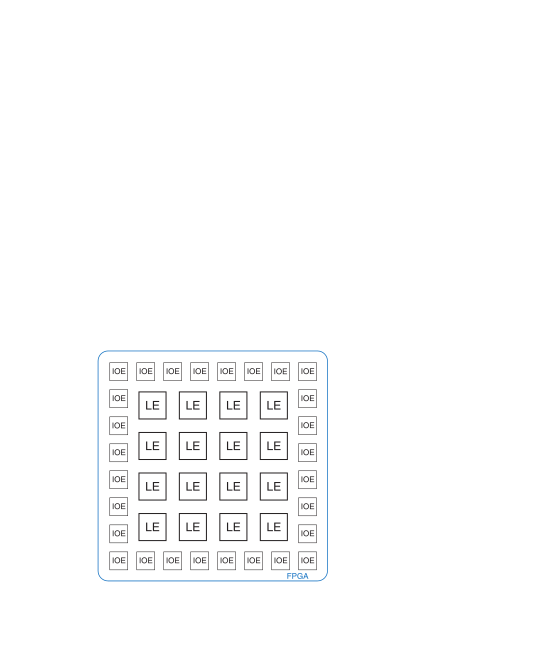
\includegraphics[width=\textwidth]{fpga.pdf}
    \caption{General \acrshort{fpga} layout \cite{harris_digital_2015}}
    \label{fig:fpga}
\end{figure} \newline \newline
%

%
\section{CNN optimizations on FPGA}
%The various optimizations can be grouped into 3 main categories, according to \textcite{abdelouahab_accelerating_2018}:
%\begin{itemize}
%    \item \textbf{Algorithmic Optimizations}: the computational cost of the convolution can be reduced by vectorizing the operation or using faster algorithms. More details can be found in section \ref{subsec:algopti}.
%    \item \textbf{Datapath Optimization}: because of the limited resources on an FPGA, memory is often the bottleneck and optimizing the memory management can increase the throughput. More details can be found in section \ref{subsec:dtptopti}.
%    \item \textbf{\acrshort{cnn} model Optimization}: an important issue of \acrshort{cnn} is their computational complexity and hardware utilization. A solution is then to use approximate computing to trade accuracy for acceleration. This work focus on this category of optimization. More details can be found in section \ref{subsec:mdopti}.
%\end{itemize}
%The following sections introduce and discuss the different optimization approaches and their various techniques.
%%%%%%%%%%%%
\section{Datapath Optimization} \label{sec:dtptopti}
blabla

%
%
\section{CNN inference on FPGA}
